\subsection{Runtime Adaptation}
\label{sec:adaptation}

\begin{figure}
  \centering
  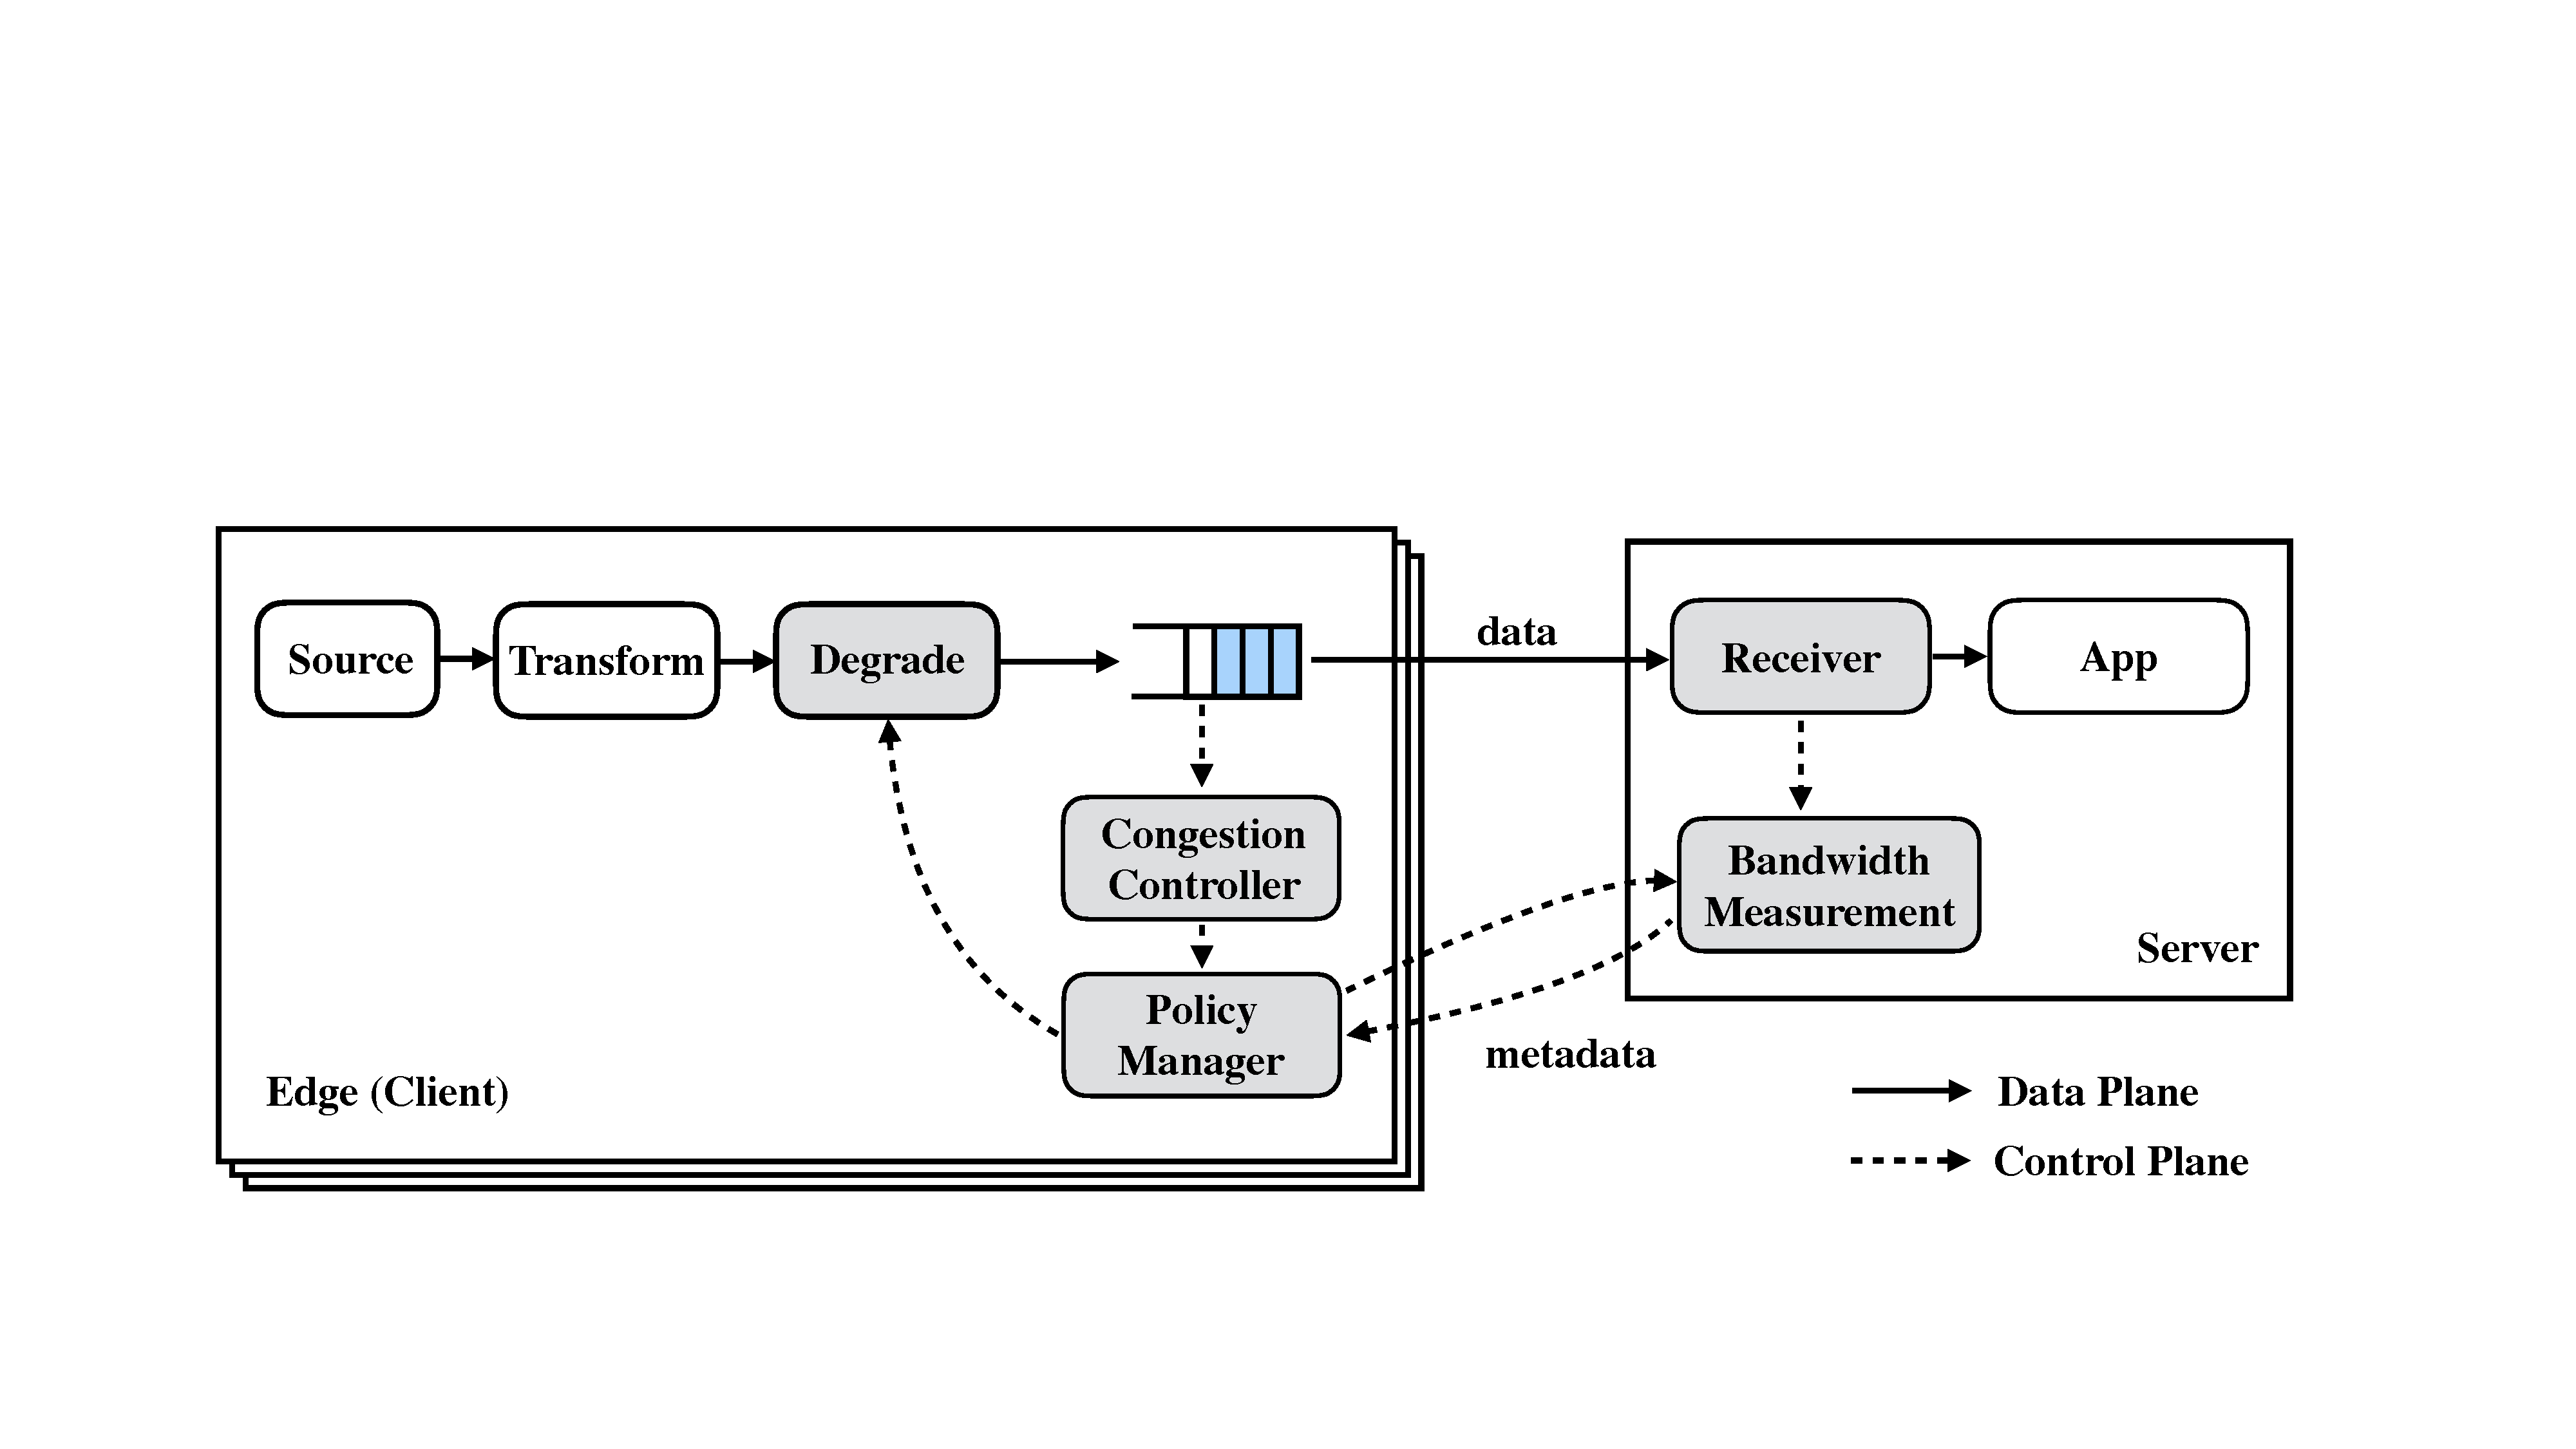
\includegraphics[width=\linewidth]{figures/runtime.pdf}
  \caption{Runtime adaptation system architecture. The grey components are what
    \sysname{} provides.}
  \label{fig:runtime}
\end{figure}

At runtime, applications automatically adapt the degradation level based on the
feedback from receiver (\autoref{fig:runtime}).

\para{Bandwidth Measurement:} The receiver measures application-level througput,
similar to \texttt{iPerf}~\cite{iperf}. To avoid sudden change, we use
exponential smoothing. To avoid unnecessary communication, the client requests
the measurement only when congestion is detected.

\para{Object-level Queue:} A queue where the unit is application object (frame).

\para{Congestion monitor:} Using a queue-based detection with high watermark and
low watermark. This can be fixed queue length, fixed data size, or estimated
queue delay based on the rate. We use the rate based.

\para{Degradation Manager:} It loads the learned profile. When receiving signals
from the congestion monitor, it adjusts the degradation level to match the
measured bandwidth. We leave some headroom here to allow queued objects being
sent. When a congestion cleared message is received, the manager increases the
rate. If some degradation operation is still in effect, after a fixed amount of
time, the manager would try to reduce the level of degradation more; until it
reaches the maximal allowed configuration.

\para{Degrade:} The actual degradation operation is rather simple. Operators
based on the \texttt{maybe} API supports a \texttt{set} function that would
change the internals of the operator. The \texttt{set} function is invoked when
degradation is needed.

%% {Interaction with TCP:} Our runtime system follow the tuning guide
%% \cite{tierney2001tcp} to adjust the send buffer.

%%% Local Variables:
%%% mode: latex
%%% TeX-master: "sigcomm2017"
%%% End:
